\documentclass{SGGW-thesis}
\usepackage{amsmath}
\usepackage{amssymb}
\usepackage{listings}
\usepackage{color}
\usepackage{xcolor}
\usepackage{amsmath}
\usepackage{graphicx}
\renewcommand{\lstlistingname}{Skrypt}

\lstset{
	basicstyle=\ttfamily\small,
	numberstyle=\tiny\color{gray},
	numbers=left,
	stepnumber=1,
	numbersep=5pt,
	frame=single,
	tabsize=2,
	captionpos=b,
	breaklines=true,
	breakatwhitespace=false,
	showspaces=false,
	showstringspaces=false,
	showtabs=false
}

\INZYNIERSKAtrue
\WZIMtrue

\title{Projekt oraz realizacja aplikacji\\wspomagającej naukę\\arytmetyki modularnej}
\Etitle{Project and implementation of an application supporting the learning of modular arithmetic}
\author{Konrad Maleńczak}
\date{2024}
\album{205844}
\thesis{Praca dyplomowa na kierunku:}
\course{Informatyka}
\promotor{dr. Andrzeja Zembrzuskiego}
\pworkplace{Instytut Informatyki Technicznej\\Katedra Systemów Informatycznych}

\usepackage{hyperref}

\begin{document}
	\maketitle
	\statementpage
	\abstractpage
	{Projekt oraz realizacja aplikacji wspomagającej naukę arytmetyki modularnej}
	{Temat tej pracy dyplomowej dotyczył zaprojektowania i implementacji aplikacji webowej wykorzystującej HTML, CSS i JavaScript, której celem było ułatwienie nauki arytmetyki modularnej dla studentów pierwszego roku informatyki na Wydziale Zastosowań Informatyki i Matematyki Szkoły Głównej Gospodarstwa Wiejskiego w Warszawie. Opisana została teoria matematyczna, implementacja wybranych algorytmów oraz wnioski.}
	{arytmetyka modularna, praca dyplomowa, implementacja, SGGW, Szkoła Główna Gospodarstwa Wiejskiego, HTML, CSS, JavaScript}
	{Project and implementation of an application supporting the learning of modular arithmetic}
	{The subject of this thesis involved the design and implementation of a web application using HTML, CSS, and JavaScript aimed at facilitating the learning of modular arithmetic for first-year computer science students at the Faculty of Applied Informatics and Mathematics of the Warsaw University of Life Sciences. The mathematical theory, implementation of selected algorithms, and conclusions were described.}
	{modular arithmetic, thesis, implementation, SGGW, Warsaw University of Life Sciences, HTML, CSS, JavaScript}
	
	{
		\doublespacing
		\tableofcontents
	}
	
	\startchapterfromoddpage
	
	\chapter{Wstęp}
	\section{Cel i zakres pracy}
	Celem tej aplikacji jest oferowanie wsparcia edukacyjnego studentom pierwszego roku informatyki w zakresie arytmetyki modularnej. Została ona zaprojektowana przy użyciu czystych technologii HTML~\cite{html}, CSS~\cite{css} i JavaScript~\cite{js}, co zapewnia jej kompatybilność zarówno z urządzeniami mobilnymi, jak i stacjonarnymi. Aplikacja charakteryzuje się intuicyjnym i~estetycznie przyjemnym interfejsem użytkownika.
	\\
	Skonstruowana z myślą o edukacji, aplikacja obejmuje osiem różnorodnych tematów, każdy z nich koresponduje z innym zagadnieniem omawianym na zajęciach z Matematyki Dyskretnej 2 dla kierunku informatyka Wydziału Zastosowań Informatyki i Matematyki Szkoły Głównej Gospodarstwa Wiejskiego w Warszawie~\cite{ajakubiec}. Każdy temat rozpoczyna się od szczegółowego wyjaśnienia teoretycznych podstaw, ilustrowanych konkretnym przykładem. Po zapoznaniu się z~teorią, użytkownicy mają możliwość przetestowania swojej wiedzy poprzez rozwiązywanie zadań na poziomie podstawowym lub zaawansowanym. Wyniki wprowadzane przez użytkownika są następnie weryfikowane przez aplikację, co pozwala na natychmiastowe otrzymanie informacji zwrotnej o ich poprawności.
	\newpage
	
	\section{Tematyka pracy}
	Praca ta skupia się na zagadnieniach arytmetyki modularnej, oferując szczegółowy wgląd w~rozumienie i implementację matematycznych problemów związanych z tą dziedziną.
	\\
	\\
	W drugim rozdziale prezentowane są fundamentalne aspekty teorii matematycznej, obejmujące działania modulo, kongruencje, algorytm Euklidesa, równania modularne, funkcję Eulera, Małe Twierdzenie Fermata, oraz Twierdzenie Eulera. Ten segment pracy stanowi solidne podstawy teoretyczne, niezbędne do dalszego zrozumienia przedstawionych koncepcji~[5-16].
	\\
	\\
	W trzecim rozdziale szczegółowo omówiona została struktura aplikacji, prezentuje jej podział na poszczególne pliki i ukazuje ich wzajemne powiązania oraz określając, które pliki odpowiadają za konkretne funkcjonalności. Ponadto, zawarto instrukcje dotyczące sposobu uruchomienia aplikacji.
	\\
	\\
	Czwarty rozdział skupia się na praktycznym zastosowaniu teorii w funkcjonowaniu aplikacji. Omówione są tu m.in. zasady działania arytmetyki modularnej, co stanowi klucz do pełnego zrozumienia mechanizmów leżących u podstaw aplikacji prezentowanej w tej pracy.
	\\
	\\
	Piąty rozdział jest poświęcony prezentacji interfejsu użytkownika aplikacji, wraz z dogłębnym opisem jego funkcjonalności. Ta część pracy dostarcza czytelnikowi wizualnego oraz funkcjonalnego zrozumienia aplikacji.
	\\
	\\
	W szóstym rozdziale, stanowiącym podsumowanie, dokonano refleksji na temat całokształtu pracy. Przedstawiono wnioski, jak również rozważania dotyczące możliwości dalszego rozwoju aplikacji, otwierając perspektywy na przyszłe badania i ulepszenia.
	\newpage
	
	\chapter{Teoria}
	Praca ma na celu stworzenie aplikacji, która wspomaga naukę arytmetyki modularnej. Niezbędna będzie do tego teoria matematyczna, która jest przedstawiona poniżej.
	\section{Operacja modulo}
	Modulo jest operacją matematyczną polegająca na wyznaczaniu reszty z dzielenia jednej liczby przez drugą. Przyjmijmy, że zapis \( a \mod d = r \) oznacza, że \( r \) jest resztą z dzielenia \( a \)~przez \( d \)~\cite{ajakubiec}\cite{r21modulo}\cite{kennweth}.
	\\
	\\
	Dzielenie z resztą można zapisać matematycznie jako:
	\begin{equation}
		a = bq + r,
	\end{equation}
	gdzie:
	\begin{itemize}
		\item \( a \) jest dzielną (reprezentuje liczbę, którą dzielimy),
		\item \( b \) jest dzielnikiem (jest to liczba, przez którą dzielimy),
		\item \( q \) jest ilorazem (wynik dzielenia),
		\item \( r \) jest resztą (jest to różnica pozostała po dzieleniu~\cite{kennweth}.
	\end{itemize}
	\vspace{1em}
	\noindent \textbf{Przykład 2.1.1} Rozpatrzmy dzielenie liczby \( 17 \) przez \( 5 \):
	\[ 17 = 5 \cdot 3 + 2 \]
	\begin{itemize}
		\item \( 17 \) to dzielna,
		\item \( 5 \) to dzielnik,
		\item \( 3 \) to iloraz,
		\item \( 2 \) to reszta.
	\end{itemize}
	
	\noindent Wynika z tego, że dzielenie \( 17 \) przez \( 5 \) daje iloraz \( 3 \) i resztę \( 2 \).
	\newpage
	
	\section{Przystawanie modulo}
	W matematyce termin \textit{kongruencje modulo}, inaczej \textit{przystawanie modulo}, odnosi się do sytuacji, kiedy dwie liczby całkowite dają tę samą resztę w procesie dzielenia przez trzecią liczbę całkowitą~\cite{ajakubiec}\cite{kennweth}\cite{lewiszax}.
	\\
	Relację \(\equiv\), czyli kongruencji, która łączy ze sobą liczby dające tę samą resztę z dzielenia przez \( n \), zapisuje się następująco:
	\begin{equation}
		a \equiv b \pmod{m},
	\end{equation}
	gdzie:
	\begin{itemize}
		\item \( a \) i \( b \) są liczbami całkowitymi,
		\item \( m \) jest liczbą całkowitą określającą operację modulo,
		\item symbol \( \equiv \) oznacza relację przystawania modulo (kongruencji)~\cite{r22modulo}\cite{lewiszax}.
	\end{itemize}
	\vspace{1em}
	\noindent \textbf{Przykład 2.2.1}
	\\
	Jako przykład weźmy liczby \( 7 \) i \( 21 \), które przystają modulo \( 7 \). Oznacza to, że obie te liczby dają tę samą resztę (\( 0 \)) przy dzieleniu przez \( 7 \). Możemy to zapisać w formie:
	\[ 7 \equiv 21 \pmod{7}. \]
	
	\noindent Wynika z tego, że liczby \( 7 \) i \( 21 \) są kongruentne w kontekście modulo \( 7 \).
	\\
	\\
	\noindent \textbf{Przykład 2.2.2}
	\\
	Rozważmy teraz liczby \( 18 \) i \( 25 \), które są przystające modulo \( 7 \). Chociaż żadna z tych liczb nie daje reszty równej \( 0 \) przy dzieleniu przez \( 7 \), to obie dają tę samą resztę \( 4 \). Możemy to zapisać jako:
	\[ 18 \equiv 25 \pmod{7}. \]
	
	\noindent Oznacza to, że liczby \( 18 \) i \( 25 \) są kongruentne w kontekście modulo \( 7 \), ponieważ obie pozostawiają resztę \( 4 \) po podzieleniu przez \( 7 \).
	\newpage
	
	\section{Działania w zbiorze reszt modulo m}
	Działania w obrębie zbioru reszt modulo \( m \) odnoszą się do operacji matematycznych z użyciem liczb całkowitych, które skutkują resztą z dzielenia tych liczb przez ustaloną liczbę całkowitą \( m \). W terminologii matematycznej, ten zbiór jest często reprezentowany jako \( \mathbb{Z}_m \)~\cite{ajakubiec}\cite{lewiszax}.
	\\
	\begin{itemize}
		\item Dodawanie w zbiorze \( \mathbb{Z}_m \): rezultat sumowania dwóch liczb całkowitych \( a \) oraz \( b \) w~kontekście modulo \( m \) przedstawia się jako:
		\begin{equation}
			(a + b) \pmod{m}.
		\end{equation}
		\textbf{Przykład 2.3.1} \( (10 + 3) \mod 4 = 13 \mod 4 = 1 \)~\cite{r23modulo}.
		\\
		\item Odejmowanie w zbiorze \( \mathbb{Z}_m \): rezultat odejmowania dwóch liczb całkowitych \( a \) oraz \( b \) w kontekście modulo \( m \) reprezentuje się jako:
		\begin{equation}
			(a - b) \pmod{m}.
		\end{equation}
		\textbf{Przykład 2.3.2} \( (10 - 3) \mod 7 = 7 \mod 7 = 0 \).
		\\
		\item Mnożenie w zbiorze \( \mathbb{Z}_m \): rezultat mnożenia dwóch liczb całkowitych \( a \) i \( b \) w kontekście modulo \( m \) określa się jako:
		\begin{equation}
			(a \cdot b) \pmod{m}.
		\end{equation}
		\textbf{Przykład 2.3.3} \( (6 \cdot 4) \mod 5 = 24 \mod 5 = 4 \).
		\\
		\item Dzielenie całkowite w zbiorze \( \mathbb{Z}_m \): wynik dzielenia całkowitego liczby \( a \) przez liczbę \( b \) w kontekście modulo \( m \) można przedstawić jako:
		\begin{equation}
			\left(\left\lfloor \frac{a}{b} \right\rfloor\right) \pmod{m}.
		\end{equation}
		\textbf{Przykład 2.3.4} \( \left\lfloor \frac{24}{4} \right\rfloor \mod 5 = 6 \mod 5 = 1. \)
	\end{itemize}
	\newpage
	
	\section{Rozszerzony algorytm Euklidesa}
	Największy wspólny dzielnik dwóch liczb całkowitych \( a \) i \( b \), zapisywany jako NWD(\( a \), \( b \)), jest największą liczbą całkowitą dzielącą bez reszty obie te liczby.
	\vspace{1em}
	\\
	\noindent Tradycyjny algorytm Euklidesa~\cite{ajakubiec}\cite{r24modulo}\cite{grygiel} jest sprawdzoną metodą ustalania największego wspólnego dzielnika (NWD) między dwoma liczbami całkowitymi. Proces ten polega na powtarzanym obliczaniu reszty z dzielenia jednej liczby przez drugą (operacja modulo), aż jedna z nich osiągnie wartość zero. W tym momencie, druga liczba reprezentuje NWD. Jest to jedna z najstarszych metod matematycznych wykorzystywanych w teorii liczb i charakteryzuje się wysoką efektywnością.
	\vspace{1em}
	\\
	Rozszerzony algorytm Euklidesa~\cite{ajakubiec}\cite{r24modulo}\cite{grygiel} jest metodą pozwalającą na obliczenie wartości zmiennych \( x \) i \( y \) w równaniu:
	\begin{equation}
		a \cdot x + b \cdot y = NWD(a, b).
	\end{equation}
	Rozszerzony algorytm Euklidesa jest użyteczny w różnych dziedzinach matematyki i informatyki. W kryptografii algorytm ten znajduje jedno ze swoich najważniejszych zastosowań, szczególnie w algorytmie RSA~\cite{rsa}, który jest jednym z najbardziej znaczących algorytmów kryptografii asymetrycznej. Ten algorytm jest kluczowym narzędziem do obliczania kluczy prywatnych i publicznych, co jest fundamentem bezpiecznej komunikacji cyfrowej.
	\\
	\\
	\noindent Rozszerzony algorytm Euklidesa jest ulepszoną formą klasycznego algorytmu, skoncentrowaną na wyznaczaniu współczynników \( x \) i \( y \) dla równania (2.7).
	\vspace{1em}
	\\
	Proces wykonywania rozszerzonego algorytmu Euklidesa obejmuje kilka kluczowych etapów:
	\begin{itemize}
		\item Rozpoczynamy od liczb \( a \) i \( b \). Należy przypisać wartość 1 do dwóch pomocniczych elementów, a dla kolejnych dwóch ustalić wartość 0 i 1.
		\item Obliczyć iloraz i resztę z dzielenia \( a \) przez \( b \), wykonując dzielenie z resztą.
		\item Zaktualizować pomocnicze elementy: pierwszy przyjmuje wartość drugiego, drugi przyjmuje wartość reszty, a następne dwa są aktualizowane w oparciu o obliczony wcześniej iloraz.
		\item Algorytm należy powtórzyć tak długo, aż nowa wartość reszty stanie się równa 0~\cite{grygiel}.
	\end{itemize}
	\newpage
	
	\noindent \textbf{Przykład 2.4.1}
	Analizujemy działanie rozszerzonego algorytmu Euklidesa dla \( n = 1547 \) i \( m = 560 \)~\cite{ajakubiec}. Najpierw należy wykonać tradycyjny algorytm Euklidesa:
	\begin{align*}
		1547 &= 2 \cdot 560 + 427 \\
		560 &= 1 \cdot 427 + 133 \\
		427 &= 3 \cdot 133 + 28 \\
		133 &= 4 \cdot 28 + 21 \\
		28 &= 1 \cdot 21 + 7 \\
		21 &= 3 \cdot 7 + 0.
	\end{align*}\\
	\noindent Z tego wynika, że NWD(1547, 560) = 7.
	\vspace{1em}
	\\
	Aby wyznaczyć współczynniki \( x \) i \( y \) w równaniu (2.7), obliczamy:
	\begin{align*}
		7 &= 28 - 1 \cdot 21 = 28 - 1 \cdot (133 - 4 \cdot 28) \\
		&= -1 \cdot 133 + 5 \cdot 28 = -1 \cdot 133 + 5 \cdot (427 - 3 \cdot 133) \\
		&= 5 \cdot 427 - 16 \cdot 133 = 5 \cdot 427 - 16 \cdot (560 - 1 \cdot 427) \\
		&= -16 \cdot 560 + 21 \cdot 427 = -16 \cdot 560 + 21 \cdot (1547 - 2 \cdot 560) \\
		&= 21 \cdot 1547 - 58 \cdot 560.
	\end{align*}
	Z tych obliczeń, z wykorzystaniem rozszerzonego algorytmu Euklidesa, wynika że:
	\[ NWD(1547, 560) = 7 = 21 \cdot 1547 - 58 \cdot 560 \]
	\newpage
	
	\section{Równania modularne}
	Istnieje wiele rodzajów kongruencji, ale jedna z najbardziej znaczących to kongruencja liniowa, opisana równaniem~\cite{r25modulo}:
	\begin{equation}
		A \cdot x \equiv B \pmod{m},
	\end{equation}
	gdzie:
	\begin{itemize}
		\item \( A \) jest współczynnikiem przy zmiennej \( x \),
		\item \( B \) jest stałą liczbą,
		\item \( m \) określa liczbę stosowaną w operacji modulo.
	\end{itemize}
	Dla \( A, B \in \mathbb{Z}, A \neq 0 \), metoda rozwiązania równania modularnego (2.8) z pojedynczą niewiadomą \( x \) przedstawiona jest poniżej~\cite{azem}.
	
	\begin{itemize}
		\item Przekształcamy dany wzór do postaci:
		\begin{equation}
			ax \equiv b \pmod{m},
		\end{equation}
		gdzie \( a \equiv A \pmod{m} \) i \( b \equiv B \pmod{m} \) przy założeniu, że \( 0 \leq a, b < m \).
		\item Następnie obliczamy największy wspólny dzielnik \( a \) i \( m \), oznaczony jako \( d = NWD(a, m) \).
		\item Sprawdzamy, czy \( d \) nie dzieli \( b \), wówczas kongruencja nie ma rozwiązania, w przeciwnym razie istnieje nieskończenie wiele rozwiązań, które wymagają dalszych obliczeń.
		\item Przeprowadzamy dzielenie przez \( d \):
		\begin{equation}
			\frac{a}{d} \cdot x \equiv \frac{b}{d} \pmod{\frac{m}{d}}.
		\end{equation}
		\item Otrzymujemy rozwiązanie:
		\begin{equation}
			x \equiv \left(\frac{a}{d}\right)^{-1} \cdot \frac{b}{d} \pmod{\frac{m}{d}}.
		\end{equation}
		\item Ustalamy odwrotność \( \left(\frac{a}{d}\right)^{-1} \) poprzez metodę prób i błędów lub korzystając z rozszerzonego algorytmu Euklidesa:
		\begin{equation}
			1 = NWD\left(\frac{a}{d}, \frac{m}{d}\right) = y \cdot \frac{a}{d} + z \cdot \frac{m}{d},
		\end{equation}
		\begin{equation}
			1 \equiv y \cdot \frac{a}{d} \pmod{\frac{m}{d}},
		\end{equation}
		\begin{equation}
			\left(\frac{a}{d}\right)^{-1} \equiv y \pmod{\frac{m}{d}}.
		\end{equation}
		\item Jedno z rozwiązań ma postać:
		\begin{equation}
			x_0 = \left(\frac{a}{d}\right)^{-1} \cdot \frac{b}{d}.
		\end{equation}
		\item Wszystkie rozwiązania można zapisać jako:
		\begin{equation}
			x = x_0 + k \cdot \frac{m}{d},
		\end{equation}
		gdzie \( k \) jest dowolną liczbą całkowitą.
	\end{itemize}
	\newpage
	
	\section{Funkcja Eulera}
	Funkcja Eulera \(\varphi\)~\cite{ajakubiec}\cite{r26modulo} przyporządkowuje każdej liczbie naturalnej liczbę liczb względnie pierwszych z nią, ale mniejszych lub równych jej samej.
	\\
	\noindent Innymi słowy, $\varphi(n)$ to liczba liczb mniejszych od $n$, które mają największy wspólny dzielnik z $n$ równy 1. Na przykład $\varphi(6) = 2$ (ponieważ tylko 1 i 5 są względnie pierwsze z 6), lub $\varphi(15) = 8$ (ponieważ liczby 1, 2, 4, 7, 8, 11, 13 i 14 są względnie pierwsze z 15).
	Funkcja Eulera, reprezentowana jako \( \varphi(n) \), odgrywa istotną funkcję w dziedzinie teorii liczb, będąc nie tylko podstawą dla Małego Twierdzenia Fermata i Twierdzenia Eulera, ale także mając zastosowanie w różnorodnych algorytmach kryptograficznych, takich jak RSA~\cite{rsa}. W innych słowach, \( \varphi(n) \) określa liczba liczb względnie pierwszych z \( n \) w zakresie od 1 do \( n \). Jest to interesujące zwłaszcza w przypadku liczb pierwszych, ponieważ dla każdej liczby pierwszej \( p \), wartość funkcji Eulera \( \varphi(p) \) równa się \( p-1 \), co jest wynikiem faktu, że wszystkie liczby mniejsze od liczby pierwszej są z nią względnie pierwsze. Na przykład liczba 13 jako liczba pierwsza jest względnie pierwsza do dwunastu liczb od 1 do 12, więc \(\varphi(13) = 12\).
	\\
	Następująca tabela wartości przedstawia wartości funkcji dla pierwszych piętnastu liczb naturalnych.
	\\
	\begin{table}[h]
		\centering
		\begin{tabular}{|c|c|c|c|c|c|c|c|c|c|c|c|c|c|c|c|}
			\hline
			$n$ & 1 & 2 & 3 & 4 & 5 & 6 & 7 & 8 & 9 & 10 & 11 & 12 & 13 & 14 & 15 \\
			\hline
			$\varphi(n)$ & 1 & 1 & 2 & 2 & 4 & 2 & 6 & 4 & 6 & 4 & 10 & 4 & 12 & 6 & 8 \\
			\hline
		\end{tabular}
		\caption{Tabela prezentująca pierwsze 15 wartości funkcji Eulera~\cite{r26modulo}.}
	\end{table}
	\\
	Obliczenie funkcji Eulera \( \varphi(n) \) wiąże się z rozkładem liczby \( n \) na czynniki pierwsze. Dokładniej, jeśli liczba \( n \) jest przedstawiona jako iloczyn potęg liczb pierwszych, tj.
	\begin{equation}
		n = \prod_{p \mid n} p^{a_p},
	\end{equation}
	gdzie \( p \) jest liczbą pierwszą, a \( a_p \) jest odpowiadającym mu wykładnikiem potęgi, wówczas wartość \( \varphi(n) \) wynika z następującego wzoru:
	\begin{equation}
		\varphi(n) = \prod_{p \mid n} p^{a_p - 1}(p - 1) = n \prod_{p \mid n} 	\left(1 - \frac{1}{p}\right).
	\end{equation}
	Oznacza to, że \( \varphi(n) \) jest iloczynem liczby \( n \) i czynników postaci \( \left(1 - \frac{1}{p}\right) \) dla każdej liczby pierwszej \( p \), która jest dzielnikiem \( n \).
	\vspace{1em}
	\\
	\noindent \textbf{Przykład 2.6.1}
	\\
	Dla \( n = 120 \), czynniki pierwsze to \( 2^3 \cdot 3^1 \cdot 5^1 \). Obliczając \( \varphi(120) \) korzystając z wzoru, otrzymujemy:
	\[ \varphi(120) = 120 \cdot \left(1 - \frac{1}{2}\right) \cdot \left(1 - \frac{1}{3}\right) \cdot \left(1 - \frac{1}{5}\right) = 120 \cdot \frac{1}{2} \cdot \frac{2}{3} \cdot \frac{4}{5} = 32. \]
	Oznacza to, że \( \varphi(120) = 32 \), co oznacza, iż 32 liczby całkowite w zakresie od 1 do 120 są względnie pierwsze z 120.
	\newpage
	
	\section{Małe Twierdzenie Fermata}
	Małe Twierdzenie Fermata~\cite{ajakubiec}\cite{r27modulo} stanowi znaczący element w teorii liczb, analizując właściwości liczb całkowitych w ramach arytmetyki modularnej, szczególnie w kontekście potęgowania. Twierdzenie to ma szerokie zastosowanie w kryptografii, teorii kodowania oraz w innych dziedzinach matematyki.
	\vspace{1em}
	\\
	\noindent Sformułowanie Małego Twierdzenia Fermata.
	\vspace{1em}
	\\
	Dla całkowitej liczby \( a \) i liczby pierwszej \( p \), obowiązuje następująca ogólna kongruencja:
	\begin{equation}
		a^p \equiv a \pmod{p}.
	\end{equation}
	Jeśli liczby \( a \) i \( p \) są względnie pierwsze, to istnieje odwrotność modulo. Innymi słowy,
	\begin{equation}
		a^{p-1} \equiv 1 \pmod{p}.
	\end{equation}
	Ogromne znaczenie tego twierdzenia odnajduje się w kryptografii, gdzie liczby pierwsze są często kluczowym elementem w generowaniu kluczy szyfrowych. Małe Twierdzenie Fermata umożliwia kontrolę zgodności z kluczami i odgrywa kluczową rolę w projektowaniu bezpiecznych systemów szyfrujących.
	\\
	\\
	\noindent \textbf{Przykład 2.7.1}
	\\
	Obliczmy \( 5^{75} \mod 13 \).
	\\
	Ponieważ \( 13 \) jest liczbą pierwszą, a \( 5 \) liczbą całkowitą, możemy zastosować Małe Twierdzenie Fermata:
	\[ 5^{12} \equiv 1 \pmod{13}, \]
	\[ 75 \mod 12 = 3, \]
	\[ 5^{75} = (5^{12})^6 \cdot 5^3 \equiv 1 \pmod{13}. \]
	Następnie obliczamy \( 5^{3} \) modulo \( 13 \):
	\[ 5^3 \equiv 8 \pmod{13}, \] 
	\[ 5^{75} \equiv (5^{12})^6 \cdot 5^3 \equiv 1^6 \cdot 8 \equiv 8 \pmod{13}. \]
	W konsekwencji, \( 5^{75} \mod 13 \) równa się \( 8 \).
	\newpage
	
	\section{Twierdzenie Eulera}
	Twierdzenie Eulera~\cite{ajakubiec}\cite{r28modulo}, znane również jako Twierdzenie Eulera-Fermata, nazwane na cześć Leonharda Eulera~[1707-1783] i Pierre'a de Fermata~[1601-1665], stanowi uogólnienie małego twierdzenia Fermata. Twierdzenie to ma zastosowanie w systemach szyfrujących, jak RSA~\cite{rsa}.
	\vspace{1em}
	\\
	\noindent Sformułowanie Twierdzenia Eulera.
	\vspace{1em}
	\\
	Dla dowolnych liczb całkowitych \( m \) i \( n \), które są wzajemnie względnie pierwsze, 
	\\
	(czyli NWD(\( m \), \( n \)) jest równy 1), zachodzi związek:
	\begin{equation}
		n^{\varphi(m)} \equiv 1 \pmod{m}.
	\end{equation}
	Warto dodać, że Twierdzenie Eulera ma znaczenie w teorii liczb oraz kryptografii, szczególnie w algorytmach bazujących na teorii liczb, takich jak RSA~\cite{rsa}. W kontekście RSA, gdzie bezpieczeństwo opiera się na trudności rozkładu na czynniki pierwsze dużych liczb pierwszych, właśnie funkcja Eulera jest wykorzystywana do generowania kluczy.
	\\
	Ponieważ dla liczb pierwszych zachodzi \( \varphi(m) = m - 1 \), w tych przypadkach Twierdzenie Eulera przechodzi w Małe Twierdzenie Fermata.
	\vspace{1em}
	\\
	\noindent \textbf{Przykład 2.8.1}
	\vspace{1em}
	\\
	Obliczmy \( 7^{85} \mod 15 \).
	\\
	Ponieważ \( 7 \) i \( 15 \) są względnie pierwsze, możemy zastosować Twierdzenie Eulera.
	\[ \varphi(15) = \varphi(3) \cdot \varphi(5) = 2 \cdot 4 = 8, \]
	\[ 7^{85} = 7^{8 \cdot 10 + 5} \equiv 7^5 \pmod{15}. \]
	Następnie obliczamy wybrane potęgi \( 7 \) modulo \( 15 \):
	\[ 7^1 \equiv 7 \pmod{15}, \]
	\[ 7^4 \equiv 4^2 = 16 \equiv 1 \pmod{15}, \]
	\[ 7^{85} \equiv 7^5 = 7^4 \cdot 7 \equiv 1 \cdot 7 = 7 \pmod{15}. \]
	Tak więc, wynik \( 7^{85} \mod 15 \) to \( 7 \).
	\newpage
	
	\chapter{Struktura aplikacji}
	W celu pełniejszego zrozumienia funkcjonalności aplikacji, kluczowe jest omówienie jej struktury. Aplikacja jest zorganizowana w sposób zapewniający łatwość nawigacji oraz intuicyjność użytkowania.
	\\
	Aplikacja zawiera łącznie czterdzieści trzy pliki, zorganizowane w precyzyjnie określonym porządku. Głównym plikiem jest \texttt{index.html}, który inicjuje działanie aplikacji. Po jego uruchomieniu użytkownikowi prezentowana jest strona główna, zawierająca wprowadzenie do arytmetyki modularnej, pasek nawigacyjny po lewej stronie oraz informacje kontaktowe twórcy aplikacji na dole strony.
	\\
	Każdy z ośmiu tematów aplikacji składa się z pięciu dedykowanych plików, a mianowicie trzech plików HTML~\cite{html} oraz dwóch plików JavaScript~\cite{js}. Pierwszy z plików HTML przedstawia teorię dotyczącą danego tematu. Dwa kolejne to strony z zadaniami - podstawowymi i zaawansowanymi. Funkcjonalności tych stron są wspierane przez przypisane im pliki JavaScript, które odpowiadają za losowanie zadań oraz weryfikację poprawności odpowiedzi użytkownika. 
	\\
	Pozostałe dwa pliki to \texttt{kontakt.html} zawierający informacje kontaktowe dostępne na każdej podstronie oraz \texttt{styles.css}~\cite{css}, odpowiadający za stylizację i układ elementów na stronie.
	\\
	Z poziomu strony głównej użytkownik może przejść do wybranego tematu, aby zgłębić jego treść teoretyczną lub rozwiązać zadania podzielone na poziomy trudności. Strony teoretyczne bezpośrednio łączą się ze stronami z zadaniami, co zapewnia płynność i przejrzystość nawigacji. Istnieje również opcja powrotu do strony głównej, aby wybrać inny temat do nauki.
	\newpage
	
	\chapter{Teoria w praktyce}
	Po zaprezentowaniu teoretycznych podstaw można przejść do opisu działania algorytmów oraz ich wdrożenia w ramach aplikacji. Każdy temat w aplikacji obejmuje zestaw czterech zadań, sklasyfikowanych jako \textit{podstawowe} i \textit{zaawansowane}. Zaleca się rozpoczynanie nauki od zadań podstawowych, ponieważ charakteryzują się one niższym poziomem trudności i stanowią doskonały punkt wyjścia. Po opanowaniu materiału podstawowego, użytkownik może przystąpić do rozwiązywania zadań zaawansowanych. Te ostatnie różnią się od poprzednich bardziej skomplikowanymi obliczeniami matematycznymi, stanowiąc wyzwanie dla bardziej zaawansowanych użytkowników.
	
	\section{Implementacja algorytmów w JavaScript}
	Algorytmy stosowane w aplikacji zostały zaimplementowane przy użyciu języka JavaScript, idealnie nadającego się do tworzenia dynamicznych aplikacji webowych~\cite{jsksiazka}. Każde z zadań obsługiwane jest przez specjalnie przygotowaną funkcję, która dostarcza rozwiązanie. W przypadku wprowadzenia przez użytkownika poprawnej odpowiedzi, na ekranie przez trzy sekundy pojawia się zielony komunikat ``Dobrze!'', zaś przy błędnej odpowiedzi wyświetlany jest czerwony komunikat ``Źle!''. Kod JavaScript jest zintegrowany z HTML, co gwarantuje poprawne wyświetlanie treści w różnych przeglądarkach internetowych. Poniższe algorytmy pochodzą z własnych źródeł i są zaimplementowane w aplikacji.

	\subsection{Inicjowanie zadań}
	Struktura kodu JavaScript skupia się na efektywnej obsłudze formularzy w aplikacji. Zadania inicjowane są przez funkcję \texttt{initializeTask}, która wykonuje następujące czynności:
	\begin{itemize}
		\item wczytywanie elementów formularza z interfejsu użytkownika,
		\item generowanie losowych danych wejściowych i ich prezentacja,
		\item ustawianie obsługi zdarzeń dla przesyłania formularza.
	\end{itemize}
	\newpage
	
	\subsection{Zarządzanie zdarzeniem przesłania formularza}
	Kolejna kluczowa funkcja, \texttt{handleTaskSubmit}, jest odpowiedzialna za:
	\begin{itemize}
		\item odbiór i analizę odpowiedzi użytkownika,
		\item ocenę poprawności udzielonych odpowiedzi,
		\item informowanie użytkownika o rezultacie jego odpowiedzi.
	\end{itemize}
	\subsection{Organizacja kodu}
	Kod programu skoncentrowany jest wokół dwóch podstawowych funkcji: \texttt{initializeTask} i \texttt{handleTaskSubmit}. Funkcja \texttt{initializeTask} aktywuje się automatycznie dla każdego z czterech zadań, gdy strona jest ładowana.
	\subsection{Proces weryfikacji odpowiedzi}
	Kod porównuje odpowiedzi użytkownika z oczekiwanymi wynikami. W zależności od poprawności odpowiedzi, wyświetlany jest odpowiedni komunikat: zielony w przypadku poprawnej odpowiedzi, a czerwony przy błędzie. Komunikat znika automatycznie po upływie trzech sekund.
	\newpage
	
	\section{Przykłady implementacji algorytmów}
	Aby skutecznie rozwiązywać zadania w aplikacji, kluczowe jest zaimplementowanie odpowiednich algorytmów. Algorytmy te stanowią fundament działania aplikacji, umożliwiając użytkownikowi interaktywne i efektywne rozwiązywanie problemów matematycznych oraz innych zadań logicznych.
	Poniżej przedstawiono wybrane algorytmy, które odegrały znaczącą rolę w procesie tworzenia aplikacji.
	
	\subsection{Algorytm generujący losowe liczby}
	Podstawowym algorytmem w aplikacji jest generator losowych liczb. Funkcja ta znacząco przyczynia się do dywersyfikacji zadań, podnosząc zarówno ich walor edukacyjny, jak i~atrakcyjność. Algorytm ten wybiera liczby losowo z określonego zakresu, zapewniając zróżnicowanie w problemach matematycznych (Skrypt 4.1).
	\vspace{1em}
	\begin{lstlisting}[caption=Funkcja generująca losowe liczby w JavaScript]
		function randomInt(min, max) {
			return Math.floor(Math.random() * (max - min + 1) + min);
		}
	\end{lstlisting}
	\vspace{1em}
	Funkcja przyjmuje dwa parametry:
	\begin{itemize}
		\item \texttt{min} - minimalna wartość zakresu (włącznie),
		\item \texttt{max} - maksymalna wartość zakresu (włącznie).
	\end{itemize}
	Wynikiem jest losowa liczba całkowita z przedziału od \texttt{min} do \texttt{max}, generowana według poniższych kroków:
	\begin{itemize}
		\item wywołanie funkcji \texttt{Math.random()} generuje liczbę zmiennoprzecinkową pomiędzy 0 a 1 (bez 1),
		\item wynik mnożony jest przez \texttt{(max - min + 1)}, co pozwala na dostosowanie zakresu do żądanych rozmiarów,
		\item dodanie wartości \texttt{min} przesuwa zakres, gwarantując, że jego dolny limit wynosi \texttt{min},
		\item na koniec, funkcja \texttt{Math.floor()} zaokrągla wynik w dół do najbliższej mniejszej liczby całkowitej, co zapewnia, że wynik pozostaje w ustalonym zakresie.
	\end{itemize}
	\newpage
	
	\subsection{Algorytm generujący losowe liczby pierwsze}
	Funkcja \texttt{randomPrime} w JavaScript jest zaprojektowana do generowania losowej liczby pierwszej w określonym przedziale. Liczby pierwsze odgrywają kluczową rolę w wielu obszarach matematyki, włączając w to kryptografię i algorytmikę (Skrypt 4.2).
	\vspace{1em}
	\begin{lstlisting}[caption=Funkcja w JavaScript do generowania liczb pierwszych]
		function randomPrime(min, max) {
			function isPrime(num) {
				if (num <= 1) return false;
				if (num <= 3) return true;
				if (num % 2 === 0 || num % 3 === 0) return false;
				let i = 5;
				while (i * i <= num) {
					if (num % i === 0 || num % (i + 2) === 0) return false;
					i += 6;
				}
				return true;
			}
			let primeNumber = randomInt(min, max);
			while (!isPrime(primeNumber)) {
				primeNumber = randomInt(min, max);
			}
			return primeNumber;
		}
	\end{lstlisting}
	\vspace{1em}
	Procedura działania funkcji \texttt{randomPrime} jest następująca:
	\begin{itemize}
		\item wewnętrzna funkcja \texttt{isPrime} ocenia, czy dana liczba \texttt{num} jest pierwsza. Sprawdza ona kryteria liczby pierwszej, czyli wyłączną podzielność przez jedynkę i samą siebie, a także, czy liczba jest większa od jedynki,
		\item centralna część funkcji \texttt{randomPrime} generuje liczbę w zakresie od \texttt{min} do \texttt{max}, a~następnie wykorzystuje \texttt{isPrime} do weryfikacji jej pierwszości,
		\item w przypadku, gdy wylosowana liczba nie jest pierwsza, proces losowania jest powtarzany do momentu uzyskania liczby pierwszej,
		\item ostatecznie funkcja zwraca wylosowaną liczbę pierwszą z zadanego przedziału.
	\end{itemize}
	\newpage
	
	\subsection{Algorytm Euklidesa do obliczania NWD}
	Obliczanie największego wspólnego dzielnika (NWD) dwóch liczb jest kluczowe w teorii liczb i ma zastosowanie w różnych dziedzinach, takich jak kryptografia, analiza numeryczna i algorytmika. NWD to największy wspólny dzielnik, który dzieli obie liczby bez reszty (Skrypt 4.3).
	\vspace{1em}
	\begin{lstlisting}[caption=Funkcja do obliczania NWD w JavaScript]
		function gcd(a, b) {
			if (b === 0) return a;
			return gcd(b, a % b);
		}
	\end{lstlisting}
	\vspace{1em}
	Proces obliczania NWD za pomocą algorytmu Euklidesa obejmuje poniższe kroki:
	\begin{itemize}
		\item algorytm rozpoczyna od sprawdzenia, czy drugi argument (\texttt{b}) jest równy \( 0 \), co stanowi warunek bazowy rekurencji,
		gdy \texttt{b} jest równy \( 0 \), zwracana jest wartość \texttt{a} jako NWD, zgodnie z definicją NWD, w przeciwnym wypadku, algorytm przechodzi do kolejnego etapu,
		\item w przypadku, gdy \texttt{b} jest różne od zera, algorytm kontynuuje poprzez rekurencyjne wywołanie funkcji \texttt{gcd},
		\item w kolejnym wywołaniu, algorytm zamienia miejscami wartości \texttt{a} i \texttt{b}, przy czym nowa wartość \texttt{b} to reszta z dzielenia \texttt{a}~przez \texttt{b},
		\item proces ten jest powtarzany aż do spełnienia warunku bazowego, czyli do momentu, gdy \texttt{b} stanie się równe 0. Wówczas aktualna wartość \texttt{a} reprezentuje NWD obu liczb.
	\end{itemize}
	\newpage
	
	\subsection{Rozszerzony algorytm Euklidesa}
	Rozszerzony algorytm Euklidesa jest rozbudowaną wersją klasycznego algorytmu obliczania NWD dwóch liczb całkowitych. Jego unikalność polega na zdolności do identyfikacji współczynników całkowitoliczbowych \(x\) i \(y\) dla danych liczb \(a\) i \(b\), które spełniają równanie \(ax + by = \text{NWD}(a, b)\). Ta funkcjonalność czyni go nieocenionym narzędziem w rozwiązaniu równań diofantycznych i w kryptografii, szczególnie w kontekście obliczania odwrotności modularnych (Skrypt 4.4).
	\vspace{1em}
	\begin{lstlisting}[caption=Funkcja Rozszerzonego Algorytmu Euklidesa w JavaScript]
		function extendedEuclideanAlgorithm(a, b) {
			let x0 = 1, y0 = 0, x1 = 0, y1 = 1;
			while (b !== 0) {
				const q = Math.floor(a / b);
				[x0, x1] = [x1, x0 - q * x1];
				[y0, y1] = [y1, y0 - q * y1];
				[a, b] = [b, a - q * b];
			}
			return [a, x0, y0];
		}
	\end{lstlisting}
	\vspace{1em}
	Algorytm inicjuje zmienne \(x0\), \(y0\), \(x1\), \(y1\) do przechowywania współczynników. Następnie, w pętli \texttt{while} wykonuje następujące operacje:
	\begin{itemize}
		\item oblicza iloraz \(q\) z dzielenia \(a\) przez \(b\),
		\item aktualizuje wartości \(x0\), \(x1\), \(y0\), \(y1\) na podstawie obliczonego ilorazu,
		\item zamienia wartości \(a\) i \(b\) dla kontynuacji algorytmu z nowymi parametrami.
	\end{itemize}
	Iteracje trwają, aż \(b\) osiągnie wartość zero. W rezultacie, algorytm zwraca NWD(\(a\), \(b\)) oraz współczynniki \(x0\) i \(y0\), które spełniają równanie \(ax + by = \text{NWD}(a, b)\).
	
	\noindent W kontekście obliczeń, algorytm rozpoczyna od sprawdzenia, czy wartość \texttt{b} jest równa 0, co stanowi warunek bazowy. Gdy \texttt{b} nie jest równe 0, algorytm wykonuje rekurencyjne wywołanie, zamieniając argumenty i stosując operację modulo. Proces ten kontynuowany jest do momentu, gdy wartość \texttt{b} stanie się równa 0, co wskazuje, że aktualna wartość \texttt{a} jest NWD obu liczb.
	\newpage
	
	\subsection{Obliczanie odwrotności modularnej}
	Odwrotność modularna to kluczowe pojęcie w teorii liczb, mające znaczenie w rozwiązywaniu kongruencji. Odwrotność modularna liczby \(a\) w module \(m\) jest to taka liczba \(x\), która spełnia równanie \(ax \equiv 1 \pmod{m}\). Rozwiązywanie kongruencji obejmuje znalezienie takich wartości \(x\), które spełniają równanie \(Ax \equiv B \pmod{m}\). Funkcje \texttt{modularInverse} i~\texttt{solveCongruence} w języku JavaScript wykonują te obliczenia.
	\vspace{1em}
	\\
	\textbf{Funkcja \texttt{modularInverse}}
	\vspace{1em}
	\\
	Odwrotność modularna liczby \(a\) w module \(m\) jest liczbą \(x\), dla której zachodzi \(ax \equiv 1 \pmod{m}\), co można zapisać jako:
	\begin{equation}
		ax \equiv 1 \pmod{m}.
	\end{equation}
	To pojęcie odgrywa istotną rolę w wielu algorytmach matematycznych i kryptograficznych, które działają w ograniczonym systemie reszt. Kod realizujący tę funkcję jest przedstawiony w skrypcie 4.5.
	\vspace{1em}
	\begin{lstlisting}[caption=Funkcja obliczająca odwrotność modularną liczby \(a\) w module \(m\) w JavaScript]
		function modularInverse(a, m) {
			a %= m;
			for (let x = 1; x < m; x++) {
				if ((a * x) % m === 1) {
					return x;
				}
			}
			return -1;
		}
	\end{lstlisting}
	\vspace{1em}
	Proces obliczania odwrotności modularnej w funkcji \texttt{modularInverse} obejmuje:
	\begin{itemize}
		\item dostosowanie wartości \(a\) do zakresu modułu \(m\),
		\item iteracyjne szukanie takiej wartości \(x\), która spełnia równanie \((a \cdot x) \mod m = 1\),
		\item zwrócenie wartości \(x\), jeśli taka istnieje. W przeciwnym razie zwrócona zostaje wartość -1.
	\end{itemize}
	\newpage
	
	\noindent \textbf{Funkcja \texttt{solveCongruence}}
	\vspace{1em}
	\\
	Znalezienie rozwiązań kongruencji liniowych jest istotnym aspektem w teorii liczb i metodach algebraicznych. Kongruencje liniowe mają postać \(Ax \equiv B \pmod{m}\), gdzie \(A\), \(B\) i \(m\) są zadanymi liczbami całkowitymi, a szukana liczba \(x\) jest niewiadomą. Proces rozwiązywania polega na odnalezieniu wszystkich możliwych wartości \(x\), które spełniają równanie w danym systemie modularnym. Kod realizujący tę funkcję jest przedstawiony w skrypcie 4.6.
	\vspace{1em}
	\begin{lstlisting}[caption=Funkcja rozwiązująca kongruencję liniową w JavaScript]
		function solveCongruence(A, B, m) {
			A %= m;
			B %= m;
			const d = gcd(A, m);
			const inv = modularInverse(A / d, m / d);
			if (B % d !== 0 || inv === -1) {
				return -1;
			} else {
				const x = (B / d) * inv;
				return x % (m / d);
			}
		}
	\end{lstlisting}
	\vspace{1em}
	Funkcja \texttt{solveCongruence} jest wykorzystywana do rozwiązywania równań kongruencji postaci \(Ax \equiv B \pmod{m}\). Jej działanie obejmuje:
	\begin{itemize}
		\item dopasowanie wartości \(A\) i \(B\) do zakresu modułu \(m\),
		\item obliczenie \( \text{NWD}(A, m) \) oraz odwrotności modularnej,
		\item weryfikację istnienia rozwiązania poprzez sprawdzenie, czy \(B\) dzieli się przez \(d\) oraz czy odwrotność modularna istnieje (czy jej wynik nie jest równy -1),
		\item jeżeli rozwiązanie istnieje, obliczenie wartości \(x\) wykorzystując odwrotność modularną, w przeciwnym razie funkcja zwraca -1,
		\item zwrócenie \(x\) jako wyniku równania kongruencji.
	\end{itemize}
	\newpage
	
	\subsection{Funkcja Eulera}
	Funkcja Eulera, znana również jako tocjent, odgrywa istotną rolę w teorii liczb. Dla każdej liczby całkowitej \( n \), funkcja Eulera, oznaczana jako \( \varphi(n) \), określa liczbę liczb całkowitych w zakresie od 1 do \( n \), które są względnie pierwsze z \( n \). Oznacza to, że zwraca liczbę liczb mniejszych od \( n \), które nie mają żadnych wspólnych dzielników z \( n \), poza liczbą 1.
	\vspace{1em}
	\begin{lstlisting}[caption=Funkcja obliczająca wartość funkcji Eulera w JavaScript]
		function eulerFunction(n) {
			let result = n;
			for (let p = 2; p * p <= n; ++p) {
				if (n % p == 0) {
					while (n % p == 0) {
						n /= p;
					}
					result -= result / p;
				}
			}
			if (n > 1) {
				result -= result / n;
			}
			return result;
		}
	\end{lstlisting}
	\vspace{1em}
	Algorytm funkcji \texttt{eulerFunction} przebiega następująco:
	\begin{itemize}
		\item początkowo zmienna \texttt{result} jest ustawiona na wartość zmiennej \( n \),
		\item funkcja iteruje przez liczby całkowite \( p \) od 2 do pierwiastka kwadratowego z \( n \), sprawdzając, czy \( p \) jest dzielnikiem \( n \),
		\item jeśli \( p \) jest dzielnikiem \( n \), to \( n \) jest dzielone przez \( p \), dopóki nie przestanie być podzielne przez \( p \). Następnie \texttt{result} jest aktualizowana przez odjęcie jej części proporcjonalnej do \( p \),
		\item jeżeli po zakończeniu pętli \( n \) pozostaje większe niż 1, oznacza to, że ma ona dzielnik pierwszy większy od jej pierwiastka kwadratowego. W tym przypadku zmienna \texttt{result} jest modyfikowana,
		\item na zakończenie, funkcja zwraca wartość \texttt{result}, będącą wynikiem \( \varphi(n) \).
	\end{itemize}
	\newpage
	
	\subsection{Potęgowanie modularne}
	Potęgowanie modularne jest podstawowym elementem teorii liczb i kryptografii, polegającym na obliczeniu reszty z dzielenia potęgi przez ustalony moduł. Ta metoda jest niezbędna w systemach modularnych, gdzie wyniki operacji muszą pozostać w określonym zakresie (Skrypt 4.8).
	\vspace{1em}
	\begin{lstlisting}[caption=Funkcja potęgowania modularnego w JavaScript]
		function calculateModuloExponentiation(base, exponent, modulus) {
			let result = 1;
			for (let i = 0; i < exponent; i++) {
				result = (result * base) % modulus;
			}
			return result;
		}
	\end{lstlisting}
	\vspace{1em}
	Działanie funkcji \texttt{calculateModuloExponentiation} obejmuje:
	\begin{itemize}
		\item inicjalizacja zmiennej \texttt{result} wartością \( 1 \),
		\item iteracyjne mnożenie \texttt{result} przez \texttt{base} (podstawę) i obliczanie reszty z dzielenia przez \texttt{modulus} po każdym mnożeniu,
		\item kontynuacja powyższego procesu aż do osiągnięcia liczby iteracji równej \texttt{exponent} (wykładnikowi),
		\item zwrócenie końcowej wartości \texttt{result}, będącej wynikiem potęgowania modularnego.
	\end{itemize}
	\newpage

	\subsection{Funkcja sprawdzająca względną pierwszość}
	Względna pierwszość liczb jest podstawowym pojęciem w teorii liczb. Mówimy, że dwie liczby są względnie pierwsze, gdy ich jedynym wspólnym dzielnikiem jest liczba 1. Ta koncepcja jest szczególnie istotna w matematyce, w tym w teorii liczb i kryptografii (Skrypt~4.9).
	\vspace{1em}
	\begin{lstlisting}[caption=Funkcja do weryfikacji względnej pierwszości w JavaScript]
		function relativelyPrime(a, b) {
			if (gcd(a, b) === 1) return true;
			return false;
		}
	\end{lstlisting}
	\vspace{1em}
	Funkcja \texttt{relativelyPrime} przeprowadza test na względną pierwszość dwóch licz całkowitych poprzez następujące kroki:
	\begin{itemize}
		\item wywołanie funkcji \texttt{gcd} do obliczenia największego wspólnego dzielnika (NWD) liczb \(a\) i \(b\),
		\item ocena, czy NWD tych liczb wynosi dokładnie \( 1 \), co jest kluczowe do stwierdzenia, że są one względnie pierwsze,
		\item zwrócenie wartości \texttt{true}, jeśli liczby są względnie pierwsze, lub \texttt{false} w przeciwnym razie.
	\end{itemize}
	\newpage
	
	\chapter{Graficzny interfejs użytkownika}
	\section{Opis ogólny}
	Aby zapewnić łatwy i uniwersalny dostęp, aplikacja została zaprojektowana do użytku w~przeglądarkach internetowych, co umożliwia jej wykorzystanie zarówno na urządzeniach stacjonarnych, jak i mobilnych. Duży nacisk położono na responsywność interfejsu, co pozwala na płynne dostosowanie się do różnych rozmiarów i rozdzielczości ekranów, co jest kluczowe dla dostępności aplikacji na urządzeniach takich jak smartfony i tablety, zwłaszcza w kontekście mobilności i dostępności edukacyjnej. W planach jest udostępnienie aplikacji poprzez jej hosting na serwerze, a także publikacja kodu źródłowego wraz z dokumentem \LaTeX \( \) na GitHubie twórcy~\cite{github}. Głównym zamierzeniem aplikacji jest wsparcie edukacyjne, szczególnie w zakresie nauki arytmetyki modularnej, która jest istotną częścią programu nauczania przedmiotu Matematyka Dyskretna 2, obowiązkowego w drugim semestrze studiów informatycznych na wydziale Zastosowań Informatyki i Matematyki w Szkole Głównej Gospodarstwa Wiejskiego w Warszawie. Uruchomienie aplikacji będzie możliwe poprzez plik \texttt{index.html}. Aplikacja składa się również z dodatkowych plików HTML, odpowiadających za różne tematy, oraz pliku \texttt{styles.css}, który zapewnia estetyczny i intuicyjny interfejs użytkownika, z odpowiednią kolorystyką, wielkością elementów oraz ich układem~\cite{htmlcssksiazka}.
	\\
	W aplikacji kluczową rolę odgrywają pliki JavaScript, które są odpowiedzialne za weryfikację poprawności obliczeń. Dla każdego zadania zaimplementowano dedykowane skrypty, które obsługują specyficzne algorytmy. Te algorytmy są niezbędne do przeprowadzania obliczeń i zapewnienia interaktywności aplikacji. W celu lepszego zobrazowania funkcjonalności aplikacji, poniżej zaprezentowane są zrzuty ekranu ilustrujące działanie poszczególnych komponentów strony.
	\newpage
	
	\section{Strona główna aplikacji}
	\begin{figure}[h]
		\centering
		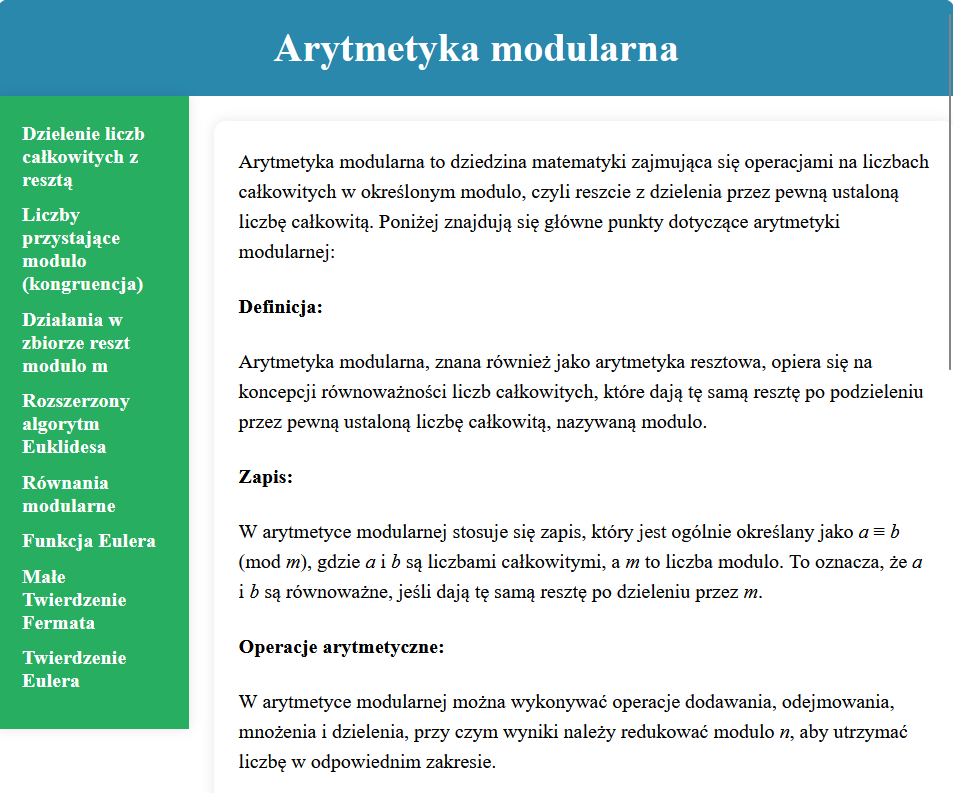
\includegraphics[width=1\textwidth]{ekranglowny.png}
		\caption{Ekran główny aplikacji. Źródło: opracowanie własne.}
		\label{fig:glowny}
	\end{figure}
	\vspace{1em}
	\noindent Strona główna aplikacji została zaprojektowana w sposób umożliwiający łatwą nawigację oraz intuicyjne zapoznanie się z podstawowymi zasadami arytmetyki modularnej. Jej układ harmonijnie łączy wstęp teoretyczny z praktycznymi aspektami nawigacji.
	\\
	Centralna część ekranu powitalnego zawiera wstęp do świata arytmetyki modularnej. Ten segment stanowi podstawę dla użytkowników, dostarczając im kluczowych informacji i wprowadzając w tematykę arytmetyki modularnej. Ta przestrzeń umożliwia użytkownikom rozpoczęcie edukacji, zapewniając podstawowe umiejętności potrzebne do dalszego zgłębiania tematu.
	Po lewej stronie ekranu znajduje się nawigacja, która umożliwia łatwe przemieszczanie się między różnymi tematami arytmetyki modularnej. Menu nawigacyjne zawiera linki do poszczególnych tematów. Ta część interfejsu użytkownika została zaprojektowana w taki sposób, aby zapewnić szybki dostęp do różnorodnych tematów, umożliwiając użytkownikom dowolność w wyborze materiału.
	\newpage
	
	\section{Strony teorii}
	\begin{figure}[h]
		\centering
		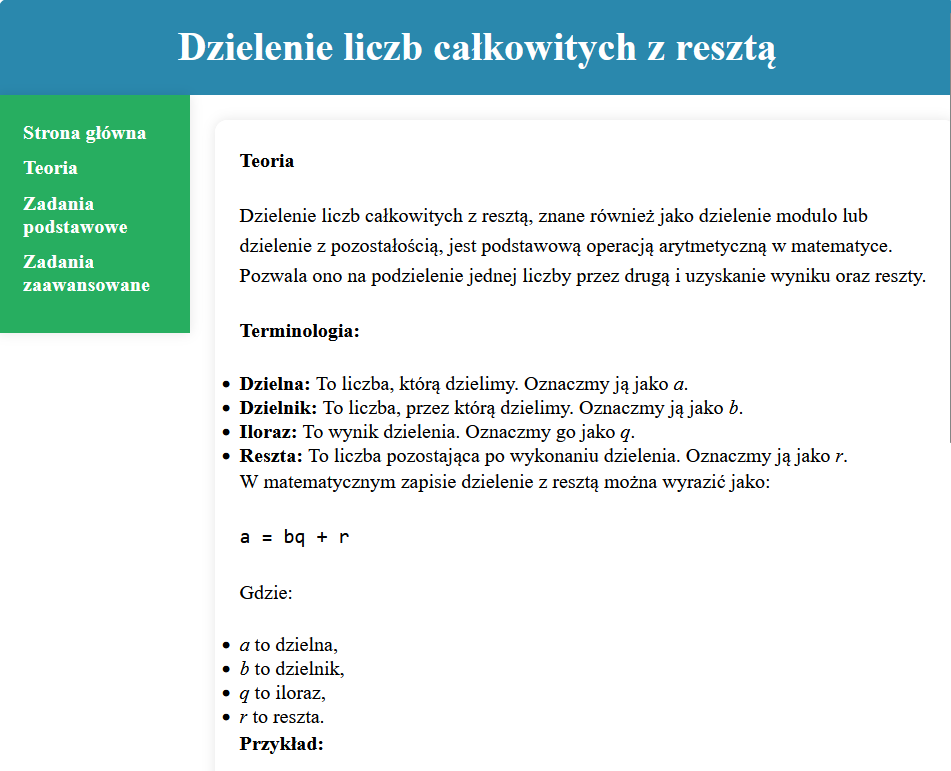
\includegraphics[width=1\textwidth]{teoria.png}
		\caption{Przykładowa strona teorii. Źródło: opracowanie własne.}
		\label{fig:teoria}
	\end{figure}
	\vspace{1em}
	\noindent Powyższa strona służy jako wszechstronny przewodnik po wybranym temacie arytmetyki modularnej, stanowiąc źródło szczegółowej wiedzy teoretycznej, precyzyjnej terminologii oraz praktycznych przykładów. Jej projekt został starannie przemyślany, aby zagwarantować użytkownikom solidne i spójne rozumienie prezentowanych zagadnień arytmetyki modularnej.
	\\
	Strona ta skrupulatnie wyjaśnia każde pojęcie i termin związany z arytmetyką modularną, od fundamentalnych definicji takich jak ``modulo", aż po bardziej skomplikowane koncepcje. Dzięki temu użytkownicy mogą z łatwością przyswajać i stosować te pojęcia w praktyce.
	\\
	\\
	\noindent \textbf{Uwaga do rysunku 5.2:} Niniejsza strona aplikacji jest jedną z ośmiu stron, która wyjaśnia teorię arytmetyki modularnej. Na rysunku jest przedstawiona przykładowa strona z~teorią.
	\newpage
	
	\section{Strony z zadaniami}
	\begin{figure}[h]
		\centering
		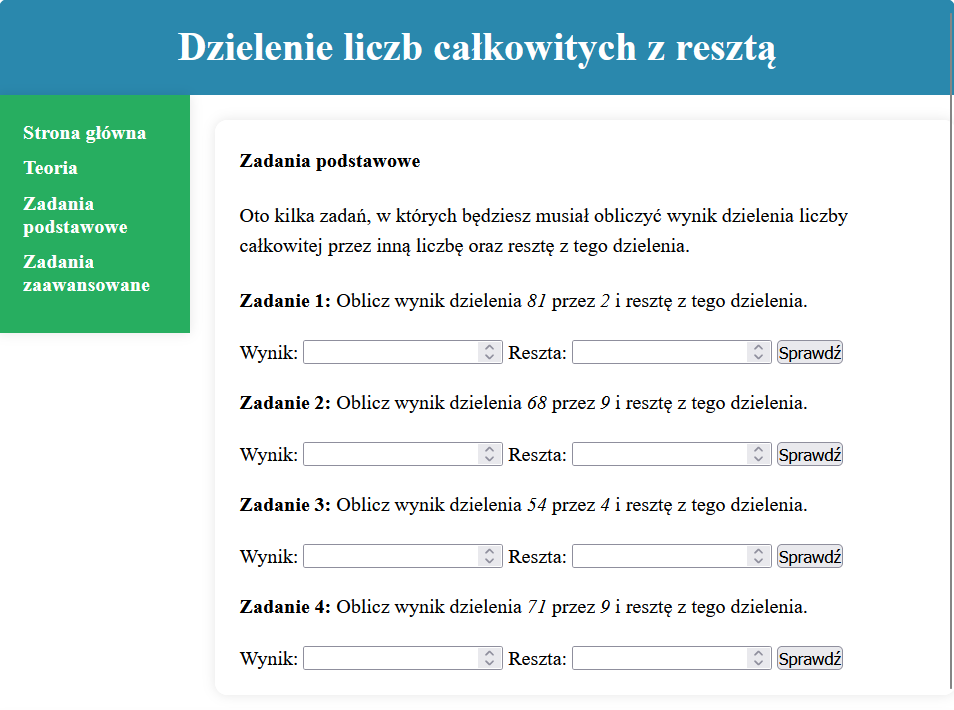
\includegraphics[width=1\textwidth]{zadania.png}
		\caption{Przykładowa strona z zadaniami podstawowymi. Źródło: opracowanie własne.}
		\label{fig:zadania}
	\end{figure}
	\vspace{1em}
	\noindent Każda z szesnastu stron z zadaniami zawiera po cztery zadania, które umożliwiają użytkownikom stosowanie i utrwalanie wiedzy z zakresu arytmetyki modularnej. Zadania te zostały opracowane, aby zapewnić praktyczne doświadczenie w rozwiązywaniu problemów i stosowaniu teorii w zadaniach. Każde z zadań jest unikalnym problemem do rozwiązania i jest przedstawione w formie formularza, umożliwiając użytkownikom wprowadzenie własnych rozwiązań i bezpośrednie otrzymanie informacji zwrotnej.
	\vspace{1em}
	\\
	\noindent W~formularzu każdego zadania znajdują się następujące elementy:
	\begin{itemize}
		\item pola wprowadzania: pola do wpisywania odpowiedzi, gdzie użytkownicy mogą wprowadzać swoje odpowiedzi do danego zadania,
		\item przycisk sprawdzenia: przycisk umożliwiający przesłanie odpowiedzi i uzyskanie natychmiastowej informacji zwrotnej,
		\item komunikat zwrotny: miejsce, w którym użytkownik otrzymuje informacje o poprawności swojej odpowiedzi. 
	\end{itemize}
	\noindent \textbf{Uwaga do rysunku 5.3:} Powyższa strona jest jedną z szesnastu stron, w tym ośmiu podstawowych i ośmiu zaawansowanych, na których można rozwiązywać zadania dotyczące arytmetyki modularnej. Na rysunku jest przedstawiona przykładowa strona z zadaniami podstawowymi.
	\newpage

	\chapter{Podsumowanie i wnioski}
	Głównym zamierzeniem przedstawionej pracy było stworzenie i wdrożenie aplikacji internetowej, mającej na celu wspieranie procesu edukacyjnego w obszarze arytmetyki modularnej. Opracowana aplikacja zapewnia wsparcie dydaktyczne dla studentów, którzy napotykają trudności w zrozumieniu matematyki na poziomie uniwersyteckim. Solidne podstawy teoretyczne, opisane na wstępie pracy, w połączeniu z opracowanymi algorytmami, zapewniają, że aplikacja efektywnie służy swoim celom edukacyjnym.
	\\
	W ramach aplikacji zaprojektowano każdy temat, uwzględniając zarówno sekcję teoretyczną, jak i praktyczne zadania. Te dwa aspekty są ze sobą nierozerwalnie powiązane, umożliwiając użytkownikom skuteczne praktykowanie i stosowanie wiedzy teoretycznej w zadaniach o zróżnicowanym stopniu trudności, od podstawowego do zaawansowanego.
	\\
	Istotnym wyzwaniem projektowym było zarządzanie strukturą plików projektu. Ostatecznie skompletowano czterdzieści trzy pliki, w tym szesnaście plików JavaScript, przeznaczonych do weryfikacji odpowiedzi użytkowników i generowania odpowiednich informacji zwrotnych. Dodatkowo, dwadzieścia sześć plików HTML odpowiada za właściwe wyświetlanie poszczególnych części aplikacji, a pojedynczy plik CSS kształtuje jej wygląd. Wszystkie te elementy wspólnie tworzą zintegrowaną całość aplikacji.
	\\
	W perspektywie rozwoju aplikacji, możliwe jest dodanie nowych funkcjonalności, takich jak kalkulator pozwalający użytkownikom na wprowadzanie i obliczanie własnych danych. Możliwe jest również rozszerzenie zakresu edukacyjnego o nowe tematy i różnorodne typy zadań. Do rozważenia jest implementacja systemu logowania do śledzenia postępów oraz wprowadzenie elementu rywalizacji między użytkownikami. Aczkolwiek, nadrzędnym celem aplikacji jest aspekt edukacyjny, co skłoniło do skupienia na doskonaleniu algorytmów i eliminacji potencjalnych niedociągnięć, kosztem implementacji dalszych funkcji.
	
	\begin{thebibliography}{10}
		\bibitem{html}
		\textit{Wikipedia. HTML.}
		\url{https://pl.wikipedia.org/wiki/HTML}
		[Dostęp 01.01.2024]
		\bibitem{css}
		\textit{Wikipedia. Kaskadowe arkusze stylów.}
		\url{https://pl.wikipedia.org/wiki/Kaskadowe_arkusze_styl%C3%B3w}
		[Dostęp 01.01.2024]
		\bibitem{js}
		\textit{Wikipedia. JavaScript.}
		\url{https://pl.wikipedia.org/wiki/JavaScript}
		[Dostęp 01.01.2024]
		\bibitem{ajakubiec}
		Jakubiec A. \textit{Prezentacje z wykładów z matematyki dyskretnej dla kierunku informatyka na Wydziale Zastosowań Informatyki i Matematyki SGGW.} 2017-2020.
		\bibitem{rsa}
		\textit{RSA (kryptografia).}
		\url{https://pl.wikipedia.org/wiki/RSA_(kryptografia)}
		[Dostęp 01.01.2024]
		\bibitem{r21modulo}
		\textit{Wikipedia. Modulo.}
		\url{https://pl.wikipedia.org/wiki/Modulo}
		[Dostęp 01.01.2024]
		\bibitem{kennweth}
		Kennweth A. Ross, Charles R.B. Wright \textit{Matematyka dyskretna.} Wydawnictwo naukowe PWN 2006, 2013, ISBN 978-83-01-14380-0.
		\bibitem{r22modulo}
		\textit{Wikipedia. Arytmetyka modularna - przystawanie.}
		\url{https://pl.wikipedia.org/wiki/Arytmetyka_modularna#Przystawanie}
		[Dostęp 01.01.2024]
		\bibitem{lewiszax}
		Lewis H., Zax R. \textit{Matematyka dyskretna. Niezbędnik dla informatyków.} Wydawnictwo naukowe PWN, 2021, ISBN 978-0-691-17929-2.
		\bibitem{r23modulo}
		\textit{Wikipedia. Arytmetyka modularna - działania.} \url{https://pl.wikipedia.org/wiki/Arytmetyka_modularna#Dzia%C5%82ania} [Dostęp 01.01.2024]
		\bibitem{r24modulo}
		\textit{Wikipedia. Algorytm Euklidesa - Rozszerzony algorytm Euklidesa.} \url{https://pl.wikipedia.org/wiki/Algorytm_Euklidesa#Rozszerzony_algorytm_Euklidesa} [Dostęp 01.01.2024]
		\bibitem{grygiel}
		Grygiel J. \textit{Wprowadzenie do matematyki dyskretnej.} Akademicka Oficyna Wydawnicza EXIT, 2007, ISBN 83-60434-26-3.
		\bibitem{r25modulo}
		\textit{Ważniak. Teoria liczb II - Rozwiązywanie równań modularnych.} \url{https://wazniak.mimuw.edu.pl/index.php?title=Matematyka_dyskretna_1/Wyk%C5%82ad_11:_Teoria_liczb_II#Rozwi%C4%85zywanie_r%C3%B3wna%C5%84_modularnych} [Dostęp 01.01.2024]
		\bibitem{azem}
		Zembrzuski A. \textit{Materiały pomocnicze do ćwiczeń z Matematyki Dyskretnej 2 na Wydziale Zastosowań Informatyki i Matematyki Szkoły Głównej Gospodarstwa Wiejskiego w Warszawie.} 2022.		\bibitem{r26modulo}
		\textit{Wikipedia. Funkcja \(\varphi\).} \url{https://pl.wikipedia.org/wiki/Funkcja_%CF%86} [Dostęp 01.01.2024]
		\bibitem{r27modulo}
		\textit{Wikipedia. Małe twierdzenie Fermata.} \url{https://pl.wikipedia.org/wiki/Ma%C5%82e_twierdzenie_Fermata} [Dostęp 01.01.2024]
		\bibitem{r28modulo}
		\textit{Wikipedia. Twierdzenie Eulera.} \url{https://pl.wikipedia.org/wiki/Twierdzenie_Eulera_(teoria_liczb)} [Dostęp 01.01.2024]
		\bibitem{jsksiazka}
		Thau D. JavaScript. \textit{Podręcznik tworzenia interaktywnych stron internetowych. Wydanie II.} Helion, 2007, ISBN 978-83-246-1079-2.
		\bibitem{github}
		\textit{GitHub.} Odnośnik do konta z pracą. \url{https://github.com/konradmal} [Dostęp 01.01.2024]
		\bibitem{htmlcssksiazka}
		Duckett J. \textit{HTML i CSS. Zaprojektuj i zbuduj witrynę WWW. Podręcznik Front-End Developera.} Helion, 2011, ISBN 978-83-283-4481-5.
	\end{thebibliography}
	
	\beforelastpage
	
\end{document}